\chapter{Our representation for trips over public transportation networks}
\label{sec:newctr}

	This is about a representation that was designed for buses.
	
	Here we speak about \gls{ttctr} and \gls{xctr}, where we have a network description and index journeys instead of explicit times. \gls{tm} as a DW-like structure.
	
	We also have lots of experimental results! Briefly mention how this is going to be plugged into the next part.
	
\section{Description}
    \label{sec:newctr:desc}
	Speak about how our network is, why another representation would lead to redundancy.
	
	Therefore, in order to better capture the information of trips over a public transportation network, and exploit this information in order to find a representation that avoids redundancy, we propose an ER model for the demand information for a public transportation network, as seen in the Figure~\ref{fig:er}.
	
	\begin{figure}[ht]
	    \begin{center}
        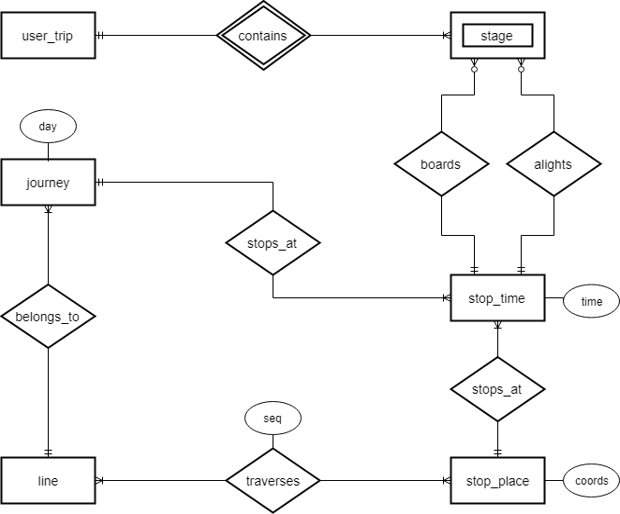
\includegraphics[width=0.75\textwidth]{figures/network_er.png}
        \caption{An ER diagram representing our model of user trips for public transportation networks.}
        \label{fig:er}
        \end{center}
    \end{figure}
    
    These are the main elements from our model:
    \begin{itemize}
        \item A \textbf{stop\_place} is a physical stop with a location, on which several lines may make stops.
        \item A \textbf{line} is an ordered sequence of stop places that can be traveled by a transport vehicle, such as a bus or a train. It only considers one travel direction. For this reason, there is often a different and complementary line for the opposite direction.%, as shown in the Figure~\ref{fig:example_network}.
        \item A \textbf{journey} is a singular traversal of a transport vehicle over a line. It can be seen as a vehicle trip, instead of a user trip.
        \item A \textbf{stage} is formed by a boarding from a stop and alighting to another from the same single line and journey.
        \item An \textbf{user\_trip} is a concatenation of several stages, until the final destination (alighting stop of the last stage) is reached.
    \end{itemize}
	
	This approach allows us to treat the information in a layered fashion: the bottom layer is a static network representation, formed by the line and stop\_place types, the middle layer represents the journeys made by vehicles that make stops at specific times, while the top layer are the trips made by the users over these vehicle journeys. Finally, it is possible to introduce a \textbf{user} identity, with an anonymized identifier to split trips by users. However, we do not consider such information useful for the kind of analysis that this work focuses on. If needed in the future, this additional entity could be trivially integrated in our representation.
	
	In order to represent and operate our data structures, we will follow this model by defining stops $s_i \in S$, lines $l_i \in L$ and journeys $j_i \in J^l$. It is important to state that journeys are \textbf{not} identified by $j_i$, as the same $j_i$ can belong to several $J^l$ from different lines, so we speak about journey \textbf{codes} (jcodes) instead of journey identifiers. In the Figure~\ref{fig:example_trips_ttctr} we can find an example network with two lines and fourteen stops, and journeys that periodically traverse these lines.
	
    \begin{figure}[ht]
        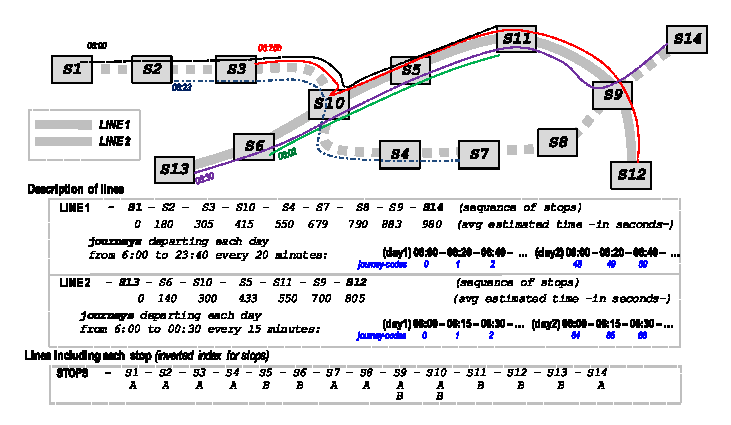
\includegraphics[width=\textwidth]{figures/network.eps}
        \caption{Network representation with the common structures.}
        \label{fig:example_trips_ttctr}
    \end{figure}
    
    A user trip can be represented by the stops from the transportation system that were boarded by a user, so from now on we will consider a trip as a sequence of triplets $<s,l,j>$, where $s$, $l$ are, respectively, stop and line identifiers, while $j$ are the journey codes corresponding to the journeys that compose the trip. These triplets describe a trip in a consecutive fashion, on the same order as the stops were boarded. Additionally, as we are interested in knowing where the trips end, we also represent the last stop where the user has alighted, which line and journey will logically match the line and journey of the last boarding stop. Although it is generally hard to obtain information about the last destination stop of a trip, many transportation companies are investing effort in providing it, either by implementing systems to keep track of users as they leave their system or estimating it based on previous trips made by that user \cite{alsger2016validating}.
    
    Example!
    
    In our first representation, \gls{ttctr}, we encode all valid $<s,l>$ pairs into a vocabulary $V$, with every trip as a concatenation of $<s,l>$ pairs for boarded stops, ended by the final destination stop, which will be alighting. We build a \gls{csa} over the concatenation of these trips, and a parallel \gls{wm} with the journey codes of the boarded stops, as previously done for \gls{ctr} in Chapter~\ref{sec:ctr}, but with a temporal component represented by line-dependant journey codes instead of explicit time intervals. For our alternative representation, \gls{xctr}, we only encode the sequence of boarded stops, while the lines go into a parallel \gls{wm}, and the journey codes are in a second \gls{wm} that is aligned to the last level of the first one, allowing us to have more flexibility for some queries, while sacrificing efficiency in others. Finally, \gls{tm} represents a matrix for each line of \texttt{stops x journeys} with the number of boardings (or alightings) performed in each cell.
	
	In the context of public transportation networks, we are interested in solving two kinds of queries, which we will present with a non-comprehensive list of examples that can be solved with the structures proposed in this work:

    \begin{enumerate}[A)]
        \item Queries about the network load, asking for the gross number of users that boarded or alighted within a stop and a time/journey. Furthermore, it can be also interesting to obtain the average load of a bus or a train between any two stops from its line. Some of those queries are:
        \begin{itemize}
            \item \boardX$_{LT}$ Number of users that stop X is boarded, optionally restricting to a line L and a time range T.
            \item \alightX$_{LT}$ Number of users that stop X is alighted, optionally restricting to a line L and a time range T.
            \item \useL$_T$  Number of users (boardings) for the line L, optionally restricting to a time range T.
            \item \boardT~Number of users boarding within a time range T.
            \item \alightT~Number of users alighting within a time range T.
            \item \loadX$_{LT}$ The average number of passengers traveling from the stop X to its next stop in the line L within the time range T. Can also be seen as the average load of the vehicle.
        \end{itemize}
        
        \item Queries about user trips patterns. With his kind of queries we can obtain the number of times a stop was used to switch lines or the number of trips that started on a stop with another specific stop as the final destination. In this work we consider the following queries of this kind:
        \begin{itemize}
            \item \startX$_{LT}$ User trips starting at a stop X, optionally restricting to a line L and a time range T.
            \item \endX$_{LT}$ User trips ending at a stop X, optionally restricting to a line L and a time range T.
            \item \switchX$_{L\textsubscript{1}L\textsubscript{2}T}$ Number of trips in which the stop X was used to switch lines, optionally restricting to a line L\textsubscript{2} and a time range T.
            \item \texttt{from\_X$_{LT}$\_to\_Y$_{LT}$} User trips that originate at stop X to end at stop Y, both being optionally restricted to a line and time range.
            \item \startL$_T$ User trips starting at any stop from the line L, optionally restricting to a time range T.
            \item \endL$_T$ User trips ending at any stop from the line L, optionally restricting to a time range T.
            \item \startT~User trips starting within a time range T.
            \item \endT~User trips ending within a time range T.
        \end{itemize}
    \end{enumerate}
	
\section{Structures}
    To the best of our knowledge, there is no indexing structure that would allow to efficiently represent trajectories that could also support all the kinds of queries described in Section~\ref{sec:newctr:desc}. For this reason, we propose a solution that relies on two data structures, \gls{tm}~and~\gls{ttctr}. The former is targeted for queries of type A, solving most aggregation queries in constant time, while the later can be used for queries of type B. Finally, we introduce a more versatile alternative to \gls{ttctr}~that we call \gls{xctr}.
    
    \subsection{Common Data Structures}
    \label{sec:cs}
    Considering our network formed by stops $s_i \in S$, lines $l_i \in L$ and journeys $j_i \in J^l$, the following structures represent these elements and all our following representations will rely on them.
    
    \begin{itemize}
        \item $lineStop_i(j)$ is the $j$th stop of line $l_i$
        \item $stopLine_i(j)$ is the $j$th line that makes a stop at the stop $s_i$
        \item $avgTime_i(j)$ is the average time in seconds that it takes for a vehicle of line $l_i$ to reach its $j$th stop from the start of a journey
        \item $initialTime_i(k)$ is the starting time of the journey $j_k$ for line $l_i$
    \end{itemize}
    
    With the exception of $initialTime$, all these structures are small enough to be represented using plain fixed-length integer arrays. In the case of $initialTime$, its size naturally grows with the amount of trips that are indexed, thus there is a motivation to reduce its size, which can be easily achieved with any technique that works on posting lists or sequences of strictly increasing numbers. In our work we used a simplified Vbyte+ANS compression described in \cite{moffat2017ans} using the Zstd library\footnote{https://github.com/facebook/zstd}. In order to facilitate searches and random access, we introduced fixed-length samples on configurable intervals.
    
    An example of these structures interacting together can be found at the Algorithm~\ref{alg:jcodes}, the the function \FuncSty{lower\_bound} is a binary search that returns the index of the first occurrence that is no lesser than the queried value, while \FuncSty{upper\_bound} returns the index of the last no greater occurrence.
    
    \begin{algorithm}[ht]
    \SetKwData{l}{$l$}\SetKwData{lz}{l$_z$}\SetKwData{s}{s}\SetKwData{sz}{s$_z$}\SetKwData{ta}{t$_a$}\SetKwData{tz}{t$_z$}\SetKwData{pattern}{pattern}\SetKwData{left}{left}\SetKwData{right}{right}\SetKwData{csa}{CSA}\SetKwData{wmj}{WMJ}\SetKwData{leftzero}{left$_0$}\SetKwData{rightzero}{right$_0$}\SetKwData{i}{i}\SetKwData{z}{z}\SetKwData{ja}{j$_a$}\SetKwData{jz}{j$_z$}\SetKwData{n}{n}\SetKwData{ap}{a'}\SetKwData{zp}{z'}\SetKwData{offset}{offset}
     \SetKwFunction{GetBounds}{GetBounds}\SetKwFunction{GetJCodes}{GetJCodes}\SetKwFunction{GetCount}{GetCount}\SetKwFunction{GetPsi}{$\Psi$}\SetKwFunction{GetRangeSpecial}{GetRange$^*$}\SetKwFunction{bsearch}{binary\_search}\SetKwFunction{lbound}{lower\_bound}\SetKwFunction{ubound}{upper\_bound}
     \SetKwProg{Fn}{Function}{\string:}{}
     
     \Fn{\GetJCodes{\l,\s,\ta,\tz}}{
     \KwData{line \l, stop \s, times \ta,\tz}
     \KwResult{jcodes for \ta and \tz}
     \BlankLine
     \offset $\leftarrow$ $avgTime_{\l}(\bsearch{$lineStop_\l$, \s})$\;
     \Return{\lbound{$initialTime_\l$, \ta-\offset}, \ubound{$initialTime_\l$, \tz-\offset}}\;
     }
     
     \caption{Obtaining the codes of the journeys from the line \l that should arrive to the stop \s within the time range given by \ta and \tz.}
     \label{alg:jcodes}
    \end{algorithm}
    
    \subsection{TTCTR}
    \ttctr~was introduced in \cite{brisaboa2018new}, where the spatial component (the pairs $(s,l)$ for the stops and lines of a trip) is represented with a \texttt{CSA} where each valid pair $(s,l)$ is encoded as an integer $id$ in the input sequence $T[1..n]$ that is used to build the \texttt{CSA}.

    In this work, \ttctr~is built first by sorting all trips. If we consider that a trip is composed by $n$ of the $<s_i,l_i,j_i>,~1\leq i\leq n$ triplets previously described, where the first triplet corresponds to the first boarded stop and the last triplet corresponds to the last alighted stop (final destination), then the collection of trips is sorted by the key $s_1,s_n,l_1,j_1$. That is, trips are initially sorted by the first boarded stop identifier. If these are equal, they are then sorted by their last stop identifier, analogously followed by the line identifier and journey code of the first stop. Figure~\ref{fig:example_trips} displays an example of a correct sorting of trips.
    
    We also need an injective function to encode the pairs $(s,l)$. Consider a vocabulary $V$ such that:
    \begin{itemize}
    	\item Entry $V[0]$ is reserved for the terminator symbol $\$$.
    	\item Entries $\langle V[1],V[2], \dots V[|S|]\rangle]$ are associated to stops $s_1,s_2,\dots, s_{|S|}$ and are used to represent the final stops of the trips. That is, when a given stop $s_i$ ends a user trip, it is given $id \leftarrow s_i$.
    	\item The following $|L|$$\times$$|S|$ entries are associated to the sequence composed of the pairs $(s,l) \in S\times L$, sorted first by the stop id $s$ and later by the line id $l$. That is, entry $V[|S|+1]$ is given to $(s_1,l_1)$; $V[|S|+2]$ to $(s_1,l_2)$; $V[|S|+3]$ to $(s_1,l_3)$; $\dots$; $V[|S|+|L|]$ to $(s_1,l_{|L|})$;  $V[|S|+|L|+1]$ to $(s_2, l_1)$, $V[|S|+|L|+2]$ to $(s_2, l_2)$, and so on. Therefore, it is easy to see that any $(s_i,l_j)$ is going to be associated to the entry $V[|S|+ |L|(i-1) + j]$.
    \end{itemize}
    
    While this arrangement would theoretically produce many entries in $V$ that are mapped to pairs $(s,l)$ that are unused in $T$, either because the stop is never traversed by that line or because we do not have the record of a user trip containing it, these entries can be skipped with a compact bitvector $B$ with rank and select capabilities, that marks with a one every used entry from $V$. This will enable us to operate with a much smaller vocabulary $V'$ with only the used entries from $V$, such that $V[i] = V'[rank_1(B,i)]$. Refer to the vocabulary shown Figure~\ref{fig:ttctr}(2) for an example where pairs $s:l$ are encoded to 43 unique identifiers in $V$. After that, $B$ marks which of the entries of $V$ actually appear in the original sequence. Finally $V'$ will contain only 12 entries, for each set bit from $B$. Note that neither $V$ nor $V'$ are explicitly represented in practice, as $rank$ and $select$ operations over $B$ are enough to map and unmap, respectively, vocabulary identifiers.

    \begin{figure}[ht]
        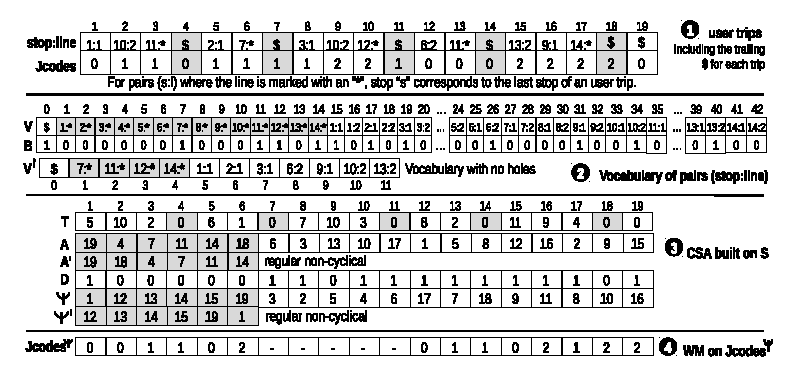
\includegraphics[width=1.00\textwidth]{figures/ttctr2019.eps}
    	\caption{Structures involved in the creation of a \acrshort{ttctr}.}
    	\label{fig:ttctr}
    \end{figure}
    
    After this, the sequence $T[1,n]$ is built, with the identifiers obtained from mapping mapping to the vocabulary entries of $V'$, over which a \texttt{CSA} is built, as seen in Figure~\ref{fig:ttctr}(3). Each encoded trip in $T$ is terminated with with additional $\$$ symbols. While in the final \texttt{CSA} we assign all these $\$$ a lexicographical value of 0 $(V[0])$, we assign them different values during the construction of the suffix array (A) to ensure that the entries for $\$$ in $A$ maintain the same order as in the original text. Finally, we make a modification on $\Psi$ to make the entries of each $\$$ point to the start of its own trip instead of the next one. These two modifications are proven necessary for our implemented queries, at the expense of losing some of the properties of a classic CSA. For reference, in Figure~\ref{fig:ttctr} we also present $A'$ and $\Psi'$, that show how our modifications compare to the original CSA.

    The journey codes ($jcodes$) are encoded in $Jcodes^{\Psi}[1,n]$, as shown in Figure~\ref{fig:ttctr}(4), that is aligned to $\Psi$ instead of $T$. $Jcodes[8]= 1$ corresponds to $Jcodes^{\Psi}[14]=1$, since $A[14]=8$; $Jcodes[9]= 2$ corresponds to $Jcodes^{\Psi}[18]=2$, since $A[18]=9$; and so on. Recall that $jcodes$ are relative to their line identifiers, leading us to skip the $jcodes$ that would be aligned to the entries of $\Psi$ belonging to the final stops (represented as ``$s\!:\!*$" in $V$), as they lack line identifiers, which are in turn needed to identify a journey. Additionally, the first positions of $Jcodes^{\Psi}$, aligned with the $\$$ entries, we duplicate the same $jcodes$ as in the start of each trip.
	
    Finally, $Jcodes^{\Psi}$ is represented with a \texttt{WM}, to support the operations we need to evaluate our proposed queries while avoiding the overhead of other types of indices that are not based in compact representations.
    
    \subsection{XCTR}
    A fundamental weakness of \ttctr~is that it requires several binary search operations over the \texttt{CSA} in the following cases:
    \begin{itemize}
        \item We are interested in the number of passengers that started their trip at a stop $s$ and a time window $t_a...t_z$, but from \textbf{any line} (\texttt{start\_X$_{T}$} from Section~\ref{sec:rq}). As $jcodes$ are relative to lines, we must make a separate query for each possible pair $(X, l_i) \forall l_i \in L$.
        \item We need to restrict the line of a final stop, in queries such as \texttt{end\_X$_{L}$} or \texttt{from\_X\_to\_Y$_{L}$} (and similar variations). Because the final stops belong to separate entries of the vocabulary that do not encode line identifiers, to restrict a stop $Y\in S$ to a line $l\in L$ we need to search for every possible expanded pattern $W_l,Y...$, for every stop $W$ from the line $l$ that could have been boarded before alighting at $Y$. While it looks tempting to address this issue by modifying the design of \ttctr~so that final stops also encode line identifiers, this would in turn make queries that do not restrict the line of the final stop inefficient, and we would need to perform a new query for every combination of $(Y, l_i) \forall l_i \in L$, as in the previous case. \marginpar{\tiny Viendo los experimentos, uno se puede preguntar si no habria quedado mejor meter lineas en paradas finales...}
    \end{itemize}
    
    These weaknesses motivated us to develop a second version, \ctr, which reduces the complexity of the queries that restrict the final line, and delegates line checks on a new WM, allowing a better space-time trade-off. As in \ttctr, the input trips need to be sorted by the same criteria, but in \ctr~we use three complementary structures to represent each component of the sequence, as shown in Figure~\ref{fig:example_xctr}:
    \begin{enumerate}[(i)]
        \item An adapted Compressed Suffix Array (\texttt{CSA}) over the stop identifiers of all trips, concatenated into a string with additional terminator symbols $\$$ appended at the end of each trip. As in the \texttt{CSA} from \ttctr, we make these $\$$ symbols maintain the order of the trips and cyclical in $\Psi$. Because this time we do not encode line and stop identifiers together and \texttt{CSA} only encodes stops, there is no need for a complex vocabulary anymore.
        \item \texttt{WML}: Aligned to the entries of (i) there is a Wavelet Matrix (WM) for the line identifiers of each stop. Aligned to the $\$$ section we duplicate the starting lines of each trip. As a trivial optimization, we build a separate WM for every stop, allowing us to save space due to the fact that a single stop does not usually belong to many lines, thus the average height of these WM is no larger (and usually smaller) than the height of a single WM.
        \item \texttt{WMJ}: A WM of jcodes aligned to the leaves of (ii). Note that this makes this structure dependant on (ii), which is coherent with the fact that journey codes themselves are relative to the line identifier. In case (ii) implements the optimization described, the entries of the WM must also be rearranged to match the delimited stops.
    \end{enumerate}
    
    \begin{figure}[ht]
    \begin{center}
    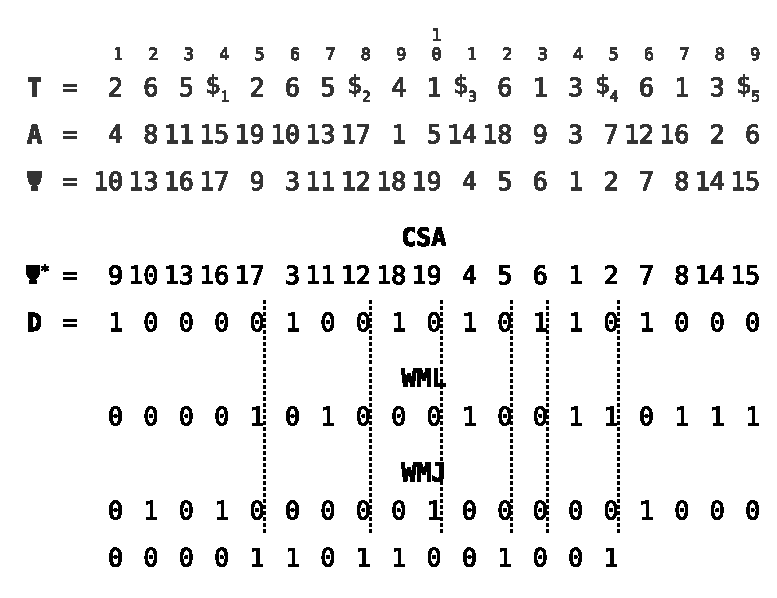
\includegraphics[width=0.8\textwidth]{figures/example_xctr.eps}
    \caption{An example of five trips represented on \ctr~with the optimizations for \texttt{WML} and \texttt{WMJ}, and sections for each stop delimited by dotted lines}
    \label{fig:example_xctr}
    \end{center}
    \end{figure}
    
    \subsection{T-Matrices}
    As it has been stated previously in this paper, nowadays it could be relatively simple to gather massive information about user trips in every public transport; however, it is not necessary to store individually each trip. If there are two (or more) travelers sharing the same bus (train/tram/etc), they are also sharing the route, the stops (the time of each stop) and even the network. Therefore, a structure storing the aggregated data of the user trips would be a handy solution to solve (at least) queries of type A presented in section 3.

    \begin{figure}[ht]
    \begin{center}
      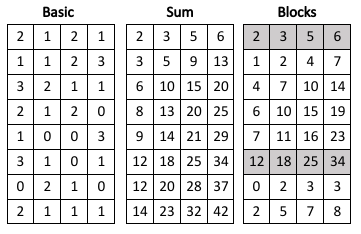
\includegraphics[scale=0.8]{figures/Tmatrices.png}
      \caption{T-Matrices example}
      \label{fig:tmatrix}
    \end{center}
    \end{figure}
    
    Thus, we propose the T-Matrix, an accumulated solution that involves two-dimensional matrices of integers enabling aggregated queries by row, column, or window/range. In the context of a public transportation network, it would be useful to solve flexible line-centered queries; that is, queries that support aggregation by any dimension. Therefore, it could be possible to aggregate either by time-interval (e.g. number of users got on at any stop of the line on 2019/01/02); by stop (e.g. number of passengers that got on a bus at stop S); or by stop and time-interval.
    
    In a na\"{\i}ve representation, it would only be necessary a two-dimensional matrix having stops as rows and journeys as columns, so each cell would have an integer representing the number of passengers that got on the vehicle at a specific stop in a particular time (journey). The main issue with this approach is that for each query it would be necessary to sum integer by integer each cell of the solution; hence, if we are trying to compute how many people got on a bus in several consecutive stops during a time interval (several consecutive journeys) it would be necessary to sum all the cells within the submatrix that match these journeys and stops.
    
    On the other hand, T-Matrix is based on this na\"{\i}ve proposal but instead of storing each cell as a simple integer it assigns an accumulated value to each slot, being the top left cell the smaller number and the bottom right position the cumulative value resulting from adding all the previous cells. Despite having larger numbers in almost every slot of the matrix, this approach allows to apply the dynamic programming formula that follows:
    
    $\mathsf{countRange((x_1,y_1),(x_2,y_2))} \leftarrow {M(x_2,y_2)} - {M(x_2,y_1-1)} - {M(x_1-1,y_2)} + {M(x_1-1,y_1-1)}$.
    
    The combination of this operations with our proposed accumulative matrix enables to compute the same two-dimensional (or one-dimensional) queries in constant time O(1), as it is only necessary to access and sum four cells in all the matrix.
    
    There are many options for compressing this cumulative matrix in order to get smaller dimensions, in this work we considered two relatively simple options with competitive results. One simple way of dealing with the growth of numbers in our cumulative solution is just apply a kind of sampling with differences; in this way, a basic example could be keep the middle column (\textit{$\mathsf{middle $\leftarrow$  (  \mathopen|c\mathclose|   + 1)/2} $}) explicitly, and representing the values in the other columns \textit{m±k} as the difference with respect to column \textit{m} (Diff in figure \ref{fig:tmatrix}). Being the algorithm to revert this differences as the one shown in Algorithm  \ref{alg:undiff}.
    
    MIDDLE FORMULA OR NOT EVEN!
    
    
    Taking this simple algorithm one step further we have built a cumulative matrix with several sampling rows, reducing significantly the size of the structure. Hence, this new differential matrix (Blocks in figure \ref{fig:tmatrix}) is divided in square blocks where the first line in each block remains the same as in the cumulative matrix while the rest of the rows in the block are calculated from it. A more technical description would be as follows in the simplified algorithm \ref{alg:unblock}.
    
    BLOCK FORMULA.


\section{Algorithms}
	A bit complex for both \gls{ttctr} and \gls{xctr}. Maybe copy the complexity table from the paper that explains why \gls{ttctr} sucks for some queries and we needed to develop \gls{xctr}.
	
	\subsection{Solving network load queries}
	Introduce jcode and \gls{tm} algorithms here!!
	
	\subsection{Solving trip pattern queries}
	With \ttctr~we obtain a clear separation between the spatial representation of the trips (\texttt{CSA}) and the temporal representation (\texttt{WM} of $jcodes$), where the former can be used to address queries such as ``number of passengers that started their trip from a stop $X\in S$ and a line $l\in L$'' (\texttt{start\_X$_{L}$} from Section~\ref{sec:rq}) with a binary search of the pattern $\$,X_l$, while the later can be used to filter down these results to a time window (\texttt{start\_X$_{LT}$}) with a $range_{a,b}(S,i,j)$ operation over the \texttt{WM}, where $a$ and $b$ are $jcodes$ obtained from Algorithm~\ref{alg:jcodes} and $i$ and $j$ delimit the range of the results obtained in $\Psi$. Because the $\$$ symbols were made cyclical in $\Psi$, it is also possible to answer \texttt{from\_X\_to\_Y} queries by searching for a pattern $Y,\$,X_l$ instead.
	
	\subsection{Analyzing our representations}
	Copy the analysis...
	
	
\section{Experiments}
	Here we compare one to the other. Maybe include query times for postgresql, maybe later.